\section{Multi-Rollen Konzept}

\subsection{Einleitung}

Um die Informationen in strongTNC zu Präsentationszwecken zugänglich machen zu können, 
ohne dass Änderungen vorgenommen werden können, weder absichtlich noch aus Versehen, 
soll eine Read-Only Rolle eingeführt werden.


\subsection{Ziel}

In einem ersten Schritt soll ein Rollen-Modell mit zwei Rollen eingeführt werden. 
Eine Rolle für Read-Only Zugriff und eine für den Vollzugriff. Der Zugriff soll, 
so wie es gegenwärtig implementiert ist, nicht personalisiert sein. Die Möglichkeit, 
den Login zu personalisieren sollte nicht grundsätzlich ausgeschlossen werden, jedoch 
steht die Implementation eines nicht personalisierten Read-Only Zugriffs im Vordergrund.


\subsection{Technische Umsetzung}

Django hat ein vollständiges Authentication- und Permission-System integriert. Damit 
lassen sich komplexe Permission-Szenarien abbilden, jedoch besteht auch die Möglichkeit 
nur Teile daraus zu verwenden und so ein einfacheres Rollen-Modell zu simulieren.

\subsubsection*{User / Permissions}

Wenn keine personalisierten Login erwünscht sind, werden zwei technische User
erstellt, die für die beiden Rollen stehen. Das heisst es gibt beispielsweise
einen User \texttt{admin-user} und einen User \texttt{readonly-user}. Dem
\texttt{admin-user} wird die Permission \texttt{write\_access} erteilt, diese
Permission kann dann mittels \texttt{@permission\_required()} Decorator geprüft
werden.

Diese Umsetzungsvariante erlaubt es mit sehr wenig Aufwand personaliserte Logins
einzuführen. Für die Verwaltung der User stellt Django ein Admin-Interface zur
Verfügung, dieses müsste also nicht selber entwickelt werden.

\subsubsection*{Templates}

In den Templates können die Permissions über das perms Objekt im Context geprüft werden. 
Beispiel:

\begin{pythoncode}

    <p>Read-write access.</p>

\end{pythoncode}

\subsubsection*{Alternativen}

Als Alternative zum Permission-System könnten auch die standardmässig vorhandenen Flags 
\texttt{user.is\_admin} und \texttt{user.is\_staff} verwendet werden. Dies wäre bedeutend 
einfacher zu implementieren, die Lösung ist jedoch nicht ausbaufähig. Deshalb wird das 
Permission-System bevorzugt.


\subsection{Frontend Änderungen}
Folgende Änderungen müssen im User Interface vorgenommen werden.

\subsubsection*{Login Screen}

Es muss eine Auswahl für die gewünschte Rolle zur Verfügung stehen. Diese kann bei zwei fix 
definierten Gruppen als Dropdown realisiert werden. Optional kann auch ein Inputfeld mit einem 
Username verwendet werden. 

\begin{figure}[H]
	\centering
	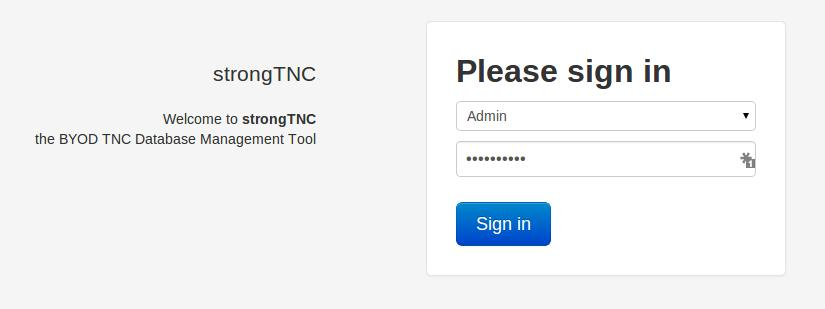
\includegraphics[width=\textwidth]{images/rollen-konzept/login-admin.jpg}
	\caption{Mögliches Aussehen der Loginmaske für den Adminlogin}
\end{figure}

\begin{figure}[H]
	\centering
	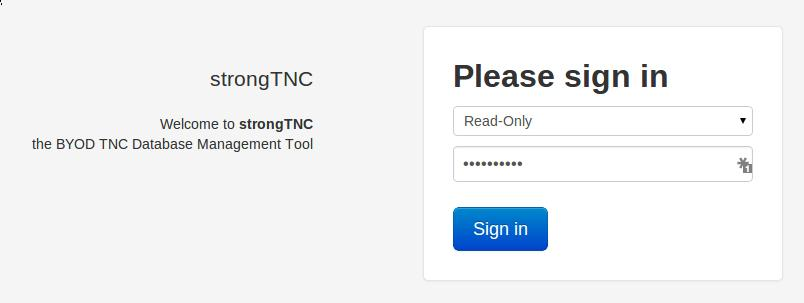
\includegraphics[width=\textwidth]{images/rollen-konzept/login-read-only.jpg}
	\caption{Mögliches Aussehen der Loginmaske für den Read-Only-Zugriff}
\end{figure}

\subsubsection{Configuration- und Data-Templates}

Alle Form-Elemente die einen Input erlauben werden deaktiviert, dies kann durch das 
Hinzufügen des HTML-Attribut \text2tt{disabled} erreicht werden. Alle Buttons werden entfernt.

\paragraph{Ausnahmen} \hspace{0pt} \\
\begin{itemize}
    \item In allen Views, das Filter-Feld
    \item In der Device-View, der Button "View device report"
\end{itemize}

\begin{figure}[H]
	\centering
	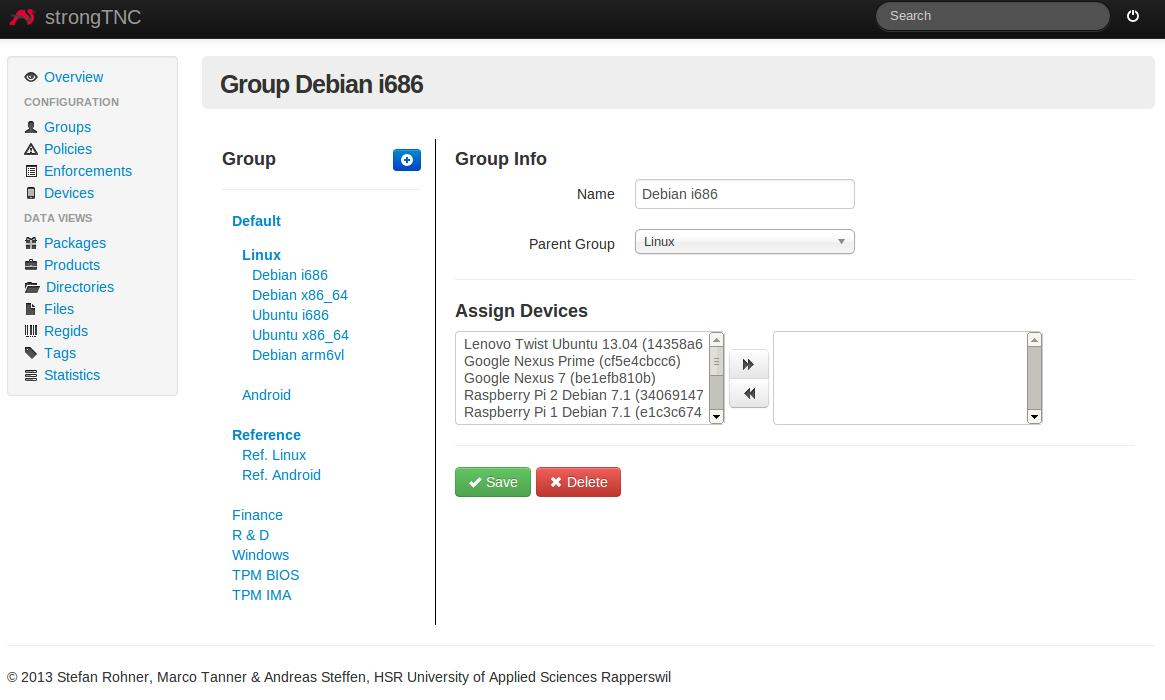
\includegraphics[width=\textwidth]{images/rollen-konzept/group-view-admin.jpg}
	\caption{Mögliches Aussehen der einer View für den Vollzugriff, am Beispiel der aktuellen Group-View}
\end{figure}

\begin{figure}[H]
	\centering
	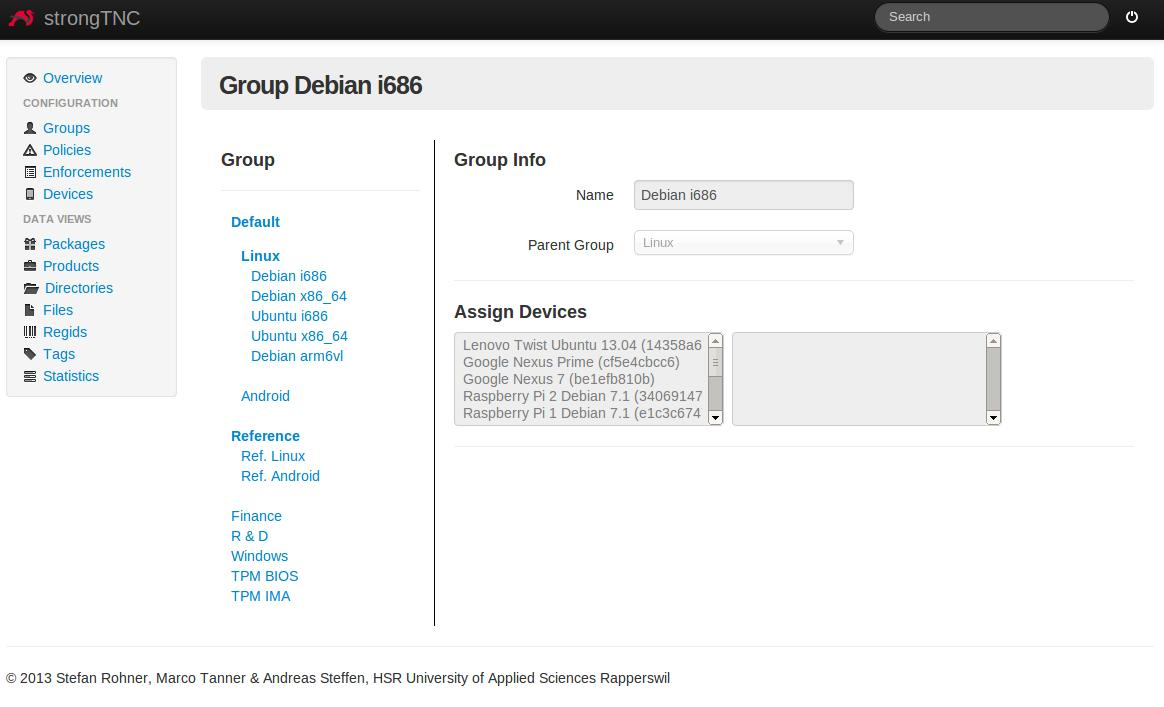
\includegraphics[width=\textwidth]{images/rollen-konzept/group-view-read-only.jpg}
	\caption{Mögliches Aussehen der einer View für den Read-Only Zugriff, am Beispiel der aktuellen Group-View}
\end{figure}


\subsection{Backend Änderungen}

Die meisten Views sind sehr ähnlich aufgebaut und verfügen über die gleichen Grundfunktionen, 
diese sind wie folgt einzuschränken:

\begin{description}
    \item [\texttt{models}] Nicht eingeschränkt
    \item [\texttt{model}] Nicht eingeschränkt
    \item [\texttt{add}] Eingeschränkt, nur für Admin
    \item [\texttt{save}] Eingeschränkt, nur für Admin
    \item [\texttt{delete}] Eingeschränkt, nur für Admin
    \item [\texttt{search}] Nicht eingeschränkt
    \item [\texttt{check}] Eingeschränkt, nur für Admin
\end{description}

Mit \texttt{models}, bzw. \texttt{models} sind die Funktionen einer View gemeint, die jeweils mit dem
Namen des Models benannt sind, zum Beispiel in der View \texttt{policy\_views.py}, die Funktionen
\texttt{policy()} und \texttt{policies()}.

\paragraph{Ausnahmen} \hspace{0pt} \\

\textbf{Device View:}
\begin{description}
    \item [\texttt{report}] Nicht eingeschränkt
    \item [\texttt{session}] Nicht eingeschränkt
\end{description}

\textbf{Package View:}
\begin{description}
    \item [\texttt{toggle\_version}] Eingeschränkt, nur für Admin
\end{description}


\section{Paketverwaltungen}


\subsubsection{DPKG}

DPKG\footnote{\url{https://alioth.debian.org/projects/dpkg}} (Abkürzung für
\textit{Debian Package}) ist die Basis der Paketverwaltung in Debian und in
verwandten Distributionen wie Ubuntu. DPKG verwaltet unter anderem alle
installierten Software-Pakete inklusive Meta-Informationen. Diese Paketliste
kann mit \texttt{dpkg-query} abgefragt werden.

\paragraph{Installierte Pakete abfragen} \hspace{0pt} \\

\noindent Mit \texttt{dpkg ---show} wird eine Liste aller installierter Pakete
ausgegeben, ein Paket pro Zeile. Um die Ausgabe zu personalisieren kann das
\texttt{---showformat} Flag verwendet werden. Im Falle des swidGenerators
ist folgendes Format ideal:

\begin{bashcode}
dpkg-query --show --showformat='${Package}\t${Version}\t${Status}\n'
\end{bashcode}

\noindent Hierbei ist noch anzumerken, dass entfernte DPKG Pakete einen sogenannten RC Status haben können. Dieser liegt vor, wenn ein Paket deinstalliert, aber die Konfigurationsdateien auf dem System belassen wurden. Die \texttt{---show} Option liefert auch diese Pakete . Dieser Der Zustand im Status Feld als \texttt{deinstall ok config-files} ersichtlich, entsprechende Pakete können so nachträglich im swidGenerator noch gefiltert werden.
\paragraph{Paket-Dateien abfragen} \hspace{0pt} \\

\noindent Um die zu einem Paket zugehörigen Dateien abzufragen, kann das
\texttt{---listfiles} Flag verwendet werden:

\begin{bashcode}
dpkg-query --listfiles <package-name>
\end{bashcode}

\paragraph{Datei-Hashes abfragen} \hspace{0pt} \\

\noindent Es besteht die Möglichkeit, aus DPKG MD5-Hashes der Dateien abzufragen. Weitere
Hash-Algorithmen (\zb SHA) sind nicht verfügbar.


\subsubsection{RPM}

RPM\footnote{\url{https://rpm.org}} (Abkürzung für
\textit{Red Hat Package Manager}) ist die Standardpaketverwaltung für Red Hat Systeme sowie zahlreichen verwandten Distributionen wie SUSE, Mandriva und Fedora.

\paragraph{Installierte Pakete abfragen} \hspace{0pt} \\

\noindent Ähnlich wie bei dpkg können alle auf dem System vorhandenen Pakete abgefragt werden. Die Ausgabe kann auch via Format String personalisiert werden. Für den swidGenerator ist folgendes Format ideal:

\begin{bashcode}
rpm -qa --queryformat %{name}\t%{version}-%{release}
\end{bashcode}

\paragraph{Paket-Dateien abfragen} \hspace{0pt} \\

\noindent Um die zu einem Paket zugehörigen Dateien abzufragen, können die Parameter \texttt{--ql} verwendet werden:

\begin{bashcode}
rpm -ql <package-name>
\end{bashcode}

\noindent TODO
